\subsection{Relative Stokes' formula (integration over the fibers)}

In this number, X and S denote two (real) manifolds of class \(C^{r}\), and \(\pi: X \to S\) a submersion. We denote by n an integer and suppose that, for every \(s \in S\), the fiber \(X_{s} = \pi^{-1}(s)\) of \(\pi\) at s (which is a submanifold of X (5.10.5)) is pure of dimension n.

11.4.1. Let E and H be two vector spaces and let F be a vector subspace of finite dimension n of H.

Let p be an integer \(\geqslant0\), u an alternating \((n+p)\)-linear map from \(H^{n+p}\) into E, and \(t_{1},\ldots,t_{p}\) elements of \(H/F\); let \(t_{1}^{\prime},\ldots,t_{p}^{\prime}\) be representatives of \(t_{1},\ldots,t_{p}\) in H. The map

\[
(x _ {1}, \dots , x _ {n}) \mapsto u (t _ {1} ^ {\prime}, \dots , t _ {p} ^ {\prime}, x _ {1}, \dots , x _ {n})
\]

is an n-linear alternating map from \(\mathbf{F}^n\) into E, which depends only on u and on the \(t_i\); it is denoted \(u \perp (t_1, \ldots, t_p)\) (cf. A, III, p. 158 for the particular case \(\mathbf{E} = \mathbf{K}\)). The map

\[
\left(t _ {1}, \dots , t _ {p}\right) \mapsto u \perp \left(t _ {1}, \dots , t _ {p}\right)
\]

is p-linear alternating.

11.4.2 (“\(\pi\)-twisted”). Consider the vector bundle \(\mathrm{T}(\mathrm{X}/\mathrm{S})\) on X (8.1.3); it has finite rank n at each point of X. We set \(\tilde{R}_{\pi} = \tilde{R}_{T(X/S)}\) (10.3.1) and \(\tilde{X}_{\pi} = \mathrm{Or}_{T(X/S)}\) (10.2.2). Let \(s \in S\); given the natural identification \(\mathrm{T}(\mathrm{X}/\mathrm{S})|_{\mathbf{X}_{s}}\) with \(\mathrm{T}(\mathbf{X}_{s})\) (8.1.3), the fiber at s of the map \(\tilde{\pi}: \tilde{X}_{\pi} \to S\), composite of \(\pi\) and the canonical map \(\tilde{X}_{\pi} \to X\), is \(\tilde{X}_{s}\) (10.2.4). A \(\pi\)-twisted differential form on X is called a \(\mathrm{T}(\mathrm{X}/\mathrm{S})\)-twisted differential form (10.3.3).

11.4.3 (“S-orientation of an S-morphism”). Let \(\mathbf{X}'\) be a variety equipped with a submersion \(\pi'\colon\mathbf{X}'\to\mathbf{S}\) whose fibers \(\mathbf{X}'_{s}\) are pure of finite dimension \(n'\), and let \(\varphi\colon\mathbf{X}'\to\mathbf{X}\) be a morphism such that \(\pi'=\pi\circ\varphi\). An S-orientation of \(\varphi\) is a morphism \(\tilde{\varphi}\colon\tilde{\mathbf{X}}'_{\pi'}\to\tilde{\mathbf{X}}_{\pi}\), commuting with the action of the group \(\{\pm1\}\) and such that the diagram

\pandocbounded{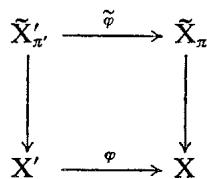
\includegraphics[keepaspectratio]{images/part001_c0391fc0.jpg}}

is commutative. The datum of an S-orientation of \(\varphi\) allows, as in 10.4.2, one to identify the bundles \(\tilde{\mathbf{R}}_{\pi'}\) and \(\varphi^{*}(\tilde{\mathbf{R}}_{\pi})\) and to define the pullback of a \(\pi\)-twisted differential form by the S-oriented morphism \(\varphi\); it is a \(\pi'\)-twisted differential form on \(\mathbf{X}'\).

11.4.4. Let A be a piece of X such that the restriction of \(\pi\) to \(\partial\mathbf{A}\) is a submersion. For every \(s\in\mathbf{S}\), the fiber \(\mathbf{X}_{s}=\pi^{-1}(s)\) is a submanifold of X transverse to \(\partial\mathbf{A}\), and \(\mathbf{A}\cap\mathbf{X}_{s}\) is a piece of \(\mathbf{X}_{s}\), denoted \(\mathbf{A}_{s}\), with boundary \(\partial\mathbf{A}\cap\mathbf{X}_{s}\).

Let \(i\) be the canonical injection of \(\partial\mathbf{A}\) into X. There exists one and only one S-orientation \(\tilde{i}\) of \(i\) such that, for every \(s\in\mathbf{S}\), the restriction of \(\tilde{i}\) to \((\partial\mathbf{A}_{s})^{\sim}\) (identified with the fiber at s of the submersion \(\partial\widetilde{\mathbf{A}}_{\pi|\partial\mathbf{A}}\to\mathbf{S}\)) is the orientation defined in 11.2.1 of the canonical injection of \(\partial\mathbf{A}_{s}\) into \(\mathbf{X}_{s}\). If \(\omega\) is a \(\pi\)-twisted differential form on X, the inverse image of \(\omega\) under the morphism \(i\) thus oriented is denoted \(\omega|\partial\mathbf{A}\) (cf. 11.2.2).

11.4.5 ("Interior product"). Let p be an integer \(\geqslant 0\) and let \(\omega\) be a \(\pi\)-twisted differential form of degree \(n + p\) on X, with values in a vector bundle E with base X. Let \(s \in S\) and \(x \in X_s\); we have \(\omega(x) = \xi \otimes u\), where \(\xi\) is an orientation of \(T_x(X_s) = T(X/S)_x\), identified with an element of \((\tilde{\mathbf{R}}_{X_s})_x = (\tilde{\mathbf{R}}_n)_x\) (10.3.2), and where u is an alternating \((n + p)\)-linear map from \(T_x(X)\) into \(E_x\). Let \(t_1, \ldots, t_p\) be tangent vectors to S at s. Put

\[
\theta (x) = \xi \otimes (u \llcorner (t _ {1}, \dots , t _ {p})) \in (\tilde {\mathbf {R}} _ {\mathrm{X} _ {s}}) _ {x} \otimes (\mathrm{Alt} ^ {n} (\mathrm{T} (\mathrm{X}); \mathrm{E})) _ {x}
\]

(cf. 11.4.1). One thus defines a twisted differential form \(\theta: x \mapsto \theta(x)\) of degree n on \(X_s\), with values in \(E|_{X_{s}}\). We denote it by \(\omega \perp (t_1, \ldots, t_p)\).

In particular, let M be a vector bundle of class \(C^{r-1}\) with base S and take \(E = \pi^{*}(M)\). The bundle \(E|_{X_{s}}\) is naturally identified with the trivial bundle with base \(X_{s}\) defined by the Banach space \(M_{s}\), and the form \(\omega\perp(t_{1},\ldots,t_{p})\) is identified with a twisted differential form on \(X_{s}\), with values in \(M_{s}\).

11.4.6. We keep the preceding notation (in particular \(E=\pi^{*}(M)\)) and assume moreover that X is separated and \(\omega\) is continuous. Let A be a piece of X such that the restriction of \(\pi\) to \(\partial A\) is a submersion and the restriction of \(\pi\) to the intersection of A and the support of \(\omega\) is proper. For \(s \in S\) and \(t_{1},\ldots,t_{p}\in\mathrm{T}_{s}(\mathrm{S})\), the form \(\omega \perp (t_{1}, \ldots, t_{p})\) (11.4.5) is a twisted differential form of degree n on \(X_{s}\), continuous, with values in the Banach space \(M_{s}\), and its support meets \(A_{s}\) in a compact set. There exists one and only one differential form \(\alpha\) of degree p on S, with values in the vector bundle M, and such that

\[
\alpha (s) \left(t _ {1}, \dots , t _ {p}\right) = \int_ {\mathrm{A} _ {s}} \omega \perp \left(t _ {1}, \dots , t _ {p}\right)
\]

for all \(s \in S\) and \(t_{1},\ldots,t_{p}\in\mathrm{T}_{s}(\mathrm{S})\). The form \(\alpha\) is denoted \(\int_{\pi|\mathbf{A}} \omega\) (or simply \(\int_{\pi} \omega\) when \(\mathbf{A} = \mathbf{X}\)); one says that it is obtained by integrating \(\omega\) over \(\mathbf{A}\) along the fibers of \(\pi\). If \(\omega\) is of class \(\mathbf{C}^{k}\) (\(0\leqslant k\leqslant r-1,\ k\leqslant\omega\)), the same is true of \(\int_{\pi|\mathbf{A}} \omega\).

When \(\omega\) is a form of degree \(< n\) , we agree that \(\int_{\pi|\mathbf{A}} \omega = 0\) .

11.4.7. We retain the preceding hypotheses and notation.

\begin{enumerate}
\def\labelenumi{\alph{enumi})}
\tightlist
\item
  For every continuous scalar differential form \(\beta\) on S, we have
\end{enumerate}

\[
\int_ {\pi | \mathrm{A}} (\pi^ {*} \beta) \wedge \omega = \beta \wedge \int_ {\pi | \mathrm{A}} \omega .
\]

\begin{enumerate}
\def\labelenumi{\alph{enumi})}
\setcounter{enumi}{1}
\tightlist
\item
  Let \(\eta\) be a continuous vector field on X and \(\zeta\) a continuous vector field on S, such that \(\eta\) is \(\pi\)-related to \(\zeta\) (8.2.6). We have
\end{enumerate}

\[
i (\zeta) \int_ {\pi | \mathrm{A}} \omega = \int_ {\pi | \mathrm{A}} i (\eta) \omega .
\]

\begin{enumerate}
\def\labelenumi{\alph{enumi})}
\setcounter{enumi}{2}
\tightlist
\item
  Suppose moreover that \(\eta\), \(\zeta\), and \(\omega\) are of class \(\mathbf{C}^1\), that \(\eta(x) \in \mathrm{T}_x(\partial \mathbf{A})\) for all \(x \in \partial \mathbf{A}\), and that \(\mathbf{M}\) is the trivial bundle defined by a Banach space E. We have
\end{enumerate}

\[
\theta_ {\zeta}. \int_ {\pi | \mathrm{A}} \omega = \int_ {\pi | \mathrm{A}} \theta_ {\eta}. \omega ,
\]

(cf. 8.4.2 and 10.3.4).

\begin{enumerate}
\def\labelenumi{\alph{enumi})}
\setcounter{enumi}{3}
\tightlist
\item
  If \(\omega\) is of degree \(n + p\) and of class \(\mathbf{C}^1\) , one has
\end{enumerate}

\[
d \left(\int_ {\pi | \mathrm{A}} \omega\right) = \int_ {\pi | \mathrm{A}} d \omega + (- 1) ^ {p} \int_ {\pi | \partial \mathrm{A}} \omega | \partial \mathrm{A}.
\]

\begin{enumerate}
\def\labelenumi{\alph{enumi})}
\setcounter{enumi}{4}
\tightlist
\item
  Suppose that S is reduced to a point. The forms \(\pi\) -twisted on X are then the ordinary twisted forms (10.4.1). If \(\omega\) is of degree \(n\) , the form \(\int_{\pi|A} \omega\) of degree 0 on S is the constant \(\int_{A} \omega\) (10.4.3).
\end{enumerate}

11.4.8. Let \(\pi': S \to S'\) be a submersion such that the fibers of \(\pi'\) are pure submanifolds of constant finite dimension \(n'\). Set \(\pi'' = \pi' \circ \pi\); it is a submersion of X onto \(S'\) whose fibers are pure submanifolds of dimension \(m = n + n'\).

Let \(x\in X\). The sequence

\[
0 \longrightarrow \mathrm{T} (\mathrm{X} / \mathrm{S}) _ {x} \stackrel {\mathrm{Id}} {\longrightarrow} \mathrm{T} (\mathrm{X} / \mathrm{S} ^ {\prime}) _ {x} \stackrel {\mathrm{T} _ {x} (\pi)} {\longrightarrow} \mathrm{T} (\mathrm{S} / \mathrm{S} ^ {\prime}) _ {\pi (x)} \longrightarrow 0
\]

is exact. There exists one and only one isomorphism \(j\) from the vector bundle \(\tilde{\mathbf{R}}_{\pi} \otimes \pi^{*}(\tilde{\mathbf{R}}_{\pi'})\) onto \(\tilde{\mathbf{R}}_{\pi'}\) such that, if \(\xi\) (resp. \(\eta\)) is an orientation of \(\mathrm{T}(\mathrm{X}/\mathrm{S})_x\) (resp. of \((\pi^{*}\mathrm{T}(\mathrm{S}/\mathrm{S}'))_x\), identified with \(\mathrm{T}(\mathrm{S}/\mathrm{S}')_{\pi(x)})\)), one has \(j(\xi \otimes \eta) = \eta\xi\) (the product being defined by the preceding exact sequence (10.2.1)).

Let M' be a vector bundle with base S'; set \(\mathbf{M} = \pi'^{*}(\mathbf{M}')\), and \(\mathbf{E}=\pi^{*}(\mathbf{M})=\pi''^{*}(\mathbf{M}')\). If \(\omega\) is a differential form that is \(\pi''\)-twisted on X with values in E, the isomorphism j allows it to be identified with a form that is \(\pi\)-twisted with values in \(\pi^{*}(\tilde{\mathbf{R}}_{\pi'}) \otimes \mathbf{E}\), or equivalently with values in \(\pi^{*}(\tilde{\mathbf{R}}_{\pi'} \otimes \mathbf{M})\).

Let A also be a piece of X such that \(\pi|\partial\mathrm{A}:\partial\mathrm{A}\to\mathrm{S}\) is a submersion; the same is then true of \(\pi''|\partial\mathrm{A}:\partial\mathrm{A}\to\mathrm{S}'\). Suppose further that \(\omega\) is continuous and that the restriction of \(\pi''\) to \(\mathbf{A}\cap\operatorname{Supp}\omega\) is proper; then the same holds for the restriction of \(\pi\) to \(\mathbf{A}\cap\operatorname{Supp}\omega\). On the one hand, one can consider the differential form \(\int_{\pi''|\mathrm{A}}\omega\) on \(\mathrm{S}'\), which is a form with values in \(\mathrm{M}'\); on the other hand, the differential form \(\int_{\pi|\mathrm{A}}\omega\) on \(\mathrm{S}\), which is a form with values in \(\tilde{\mathbf{R}}_{\pi'}\otimes\mathrm{M}\), or equivalently a \(\pi'\)-twisted form with values in \(\mathbf{M}=\pi'^{*}(\mathbf{M}')\). Moreover, \(\pi(\mathrm{A})\) is an open submanifold of \(\mathrm{S}\) and the restriction of \(\pi'\) to \(\pi(\mathrm{A})\cap\mathrm{Supp}\int_{\pi|\mathrm{A}}\omega\) is proper. The differential form \(\int_{\pi'|\pi(\mathrm{A})}\int_{\pi|\mathrm{A}}\omega\) is defined; it is a differential form on \(\mathrm{S}'\), with values in \(\mathrm{M}'\). One has

\[
\int_ {\pi^ {\prime} \circ \pi | A} \omega = \int_ {\pi^ {\prime} | \pi (A)} \int_ {\pi | A} \omega .
\]

If A = X, we have

\[
\int_ {\pi^ {\prime} \circ \pi} \omega = \int_ {\pi^ {\prime}} \int_ {\pi} \omega .
\]

